\chapter{Existing Similar Games}
\label{competitive-games}

This chapter aims to compare the~analyzed game, as described in chapter~\ref{analysis}, with existing similar educational or programming games.
Games will be compared based on criteria found in the~conducted survey and studies mentioned in the~introduction.

There is a~vast number of such different games.
There are games for the~web, desktop, mobile phones, and possibly various board games.
It is impossible to describe all types of games, so 10 representatives will be selected to represent a~broader range of such products.
Listed games are selected subjectively as the~most related and known by the~author.

The~conducted survey done in chapter~\ref{survey} found that children players are competitive, they like receiving rewards and ratings and play mostly building games.
Also, in the~article~\cite{nand_2019_engaging} they found that challenges were the~most appealing, together with feedback~-- with the~meaning that players like to be scored~-- and graphics.
In the~article~\cite{smiderle_2020_the}, similar results were shown while investigating the~influence of points, badges, and ranking.
As the~article states, \textquote{Gamified group participants had a~significant improvement in the~quality of the~submitted solutions, having obtained more accuracy.}

Therefore, this chapter will compare similar games' comprehensibility, story, study materials, graphics, and feedback.
Moreover, because the~game \emph{\myAppName} aims at young people, it will also compare their prices.

For each game, it will be described what the~player can do in the~game and what mechanisms they can use.
The~user interface and how it is handled will also be described.
In particular, the~elements that the~game does not address adequately and, conversely, the~aspects that the~game excels in will be highlighted.
The~proposed game will try to avoid inappropriate elements and inspire the~appropriate ones.

\pagebreak
\section{Scratch}
\label{similar-games:scratch}

\begin{figure}
    \centering
    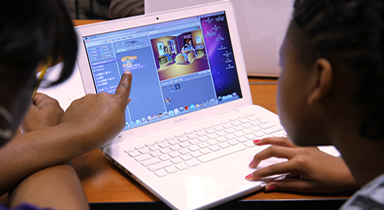
\includegraphics[width=1\linewidth]{assets/similar-games/scratch.jpg}
    \caption{Scratch~\cite{a2022_scratch}}
    \label{fig:scratch}
\end{figure}

Scratch is one of the~most extensive coding applications with a~simple visual interface that allows the~creation of universal programs, as can be seen in the~figure~\ref{fig:scratch}.

After entering the~game, a~user sees several projects of other users, which they can open and try.
If the~user opens a~game, they see a~game window, instructions for playing, and other notes and credits.
If the~user is interested in how the~game is programmed, they can see the~inside, which takes them to its editor screen.
They can then create a~remix for the~game, an~open continuation of the~original game with any modifications.

It is already clear from the~mentioned progress that the~game Scratch is focused on open creation and encourages the~creativity of its players.
The~user can create a~new game.
The~only means are the~editor's free area and the~blocks on the~window side that can be moved and combined to achieve the~desired effect -- to program the~game according to the~user's idea.

The~editor provides a~wide range of visual commands divided into several categories.
There are categories like motion, looks, sound, events, etc.
Each such category contains several visual commands that interact with the~game character or the~world differently.
These commands consist of individual blocks glued together in the~editor area.
All commands under the~current command are stuck to it, and if the~user grabs a~command, anything stuck under it will be grabbed with it.
Commands are placed anywhere in the~area, and there is no fixed grid.

\pagebreak
Players can create games, animation, and other visual creations.
That promotes problem-solving skills and collaboration.
According to~\cite{a2022_scratch}, Scratch is a~nonprofit organization, widely available in more than 70 languages, and designed for ages 8 to 16.
The~game is also completely free.

Although Scratch has no story, it does contain a~few more miniature tutorials that bring the~user closer to the~editor and its abilities.
Since the~game does not have fixed rules for the~games created, the~created games have no score for fulfillment.
The~only measure can be the~number of impressions, likes in the~form of stars and hearts, and the~number of remixes created. 

\section{Khan Academy}
\label{similar-games:khan-academy}

\begin{figure}
    \centering
    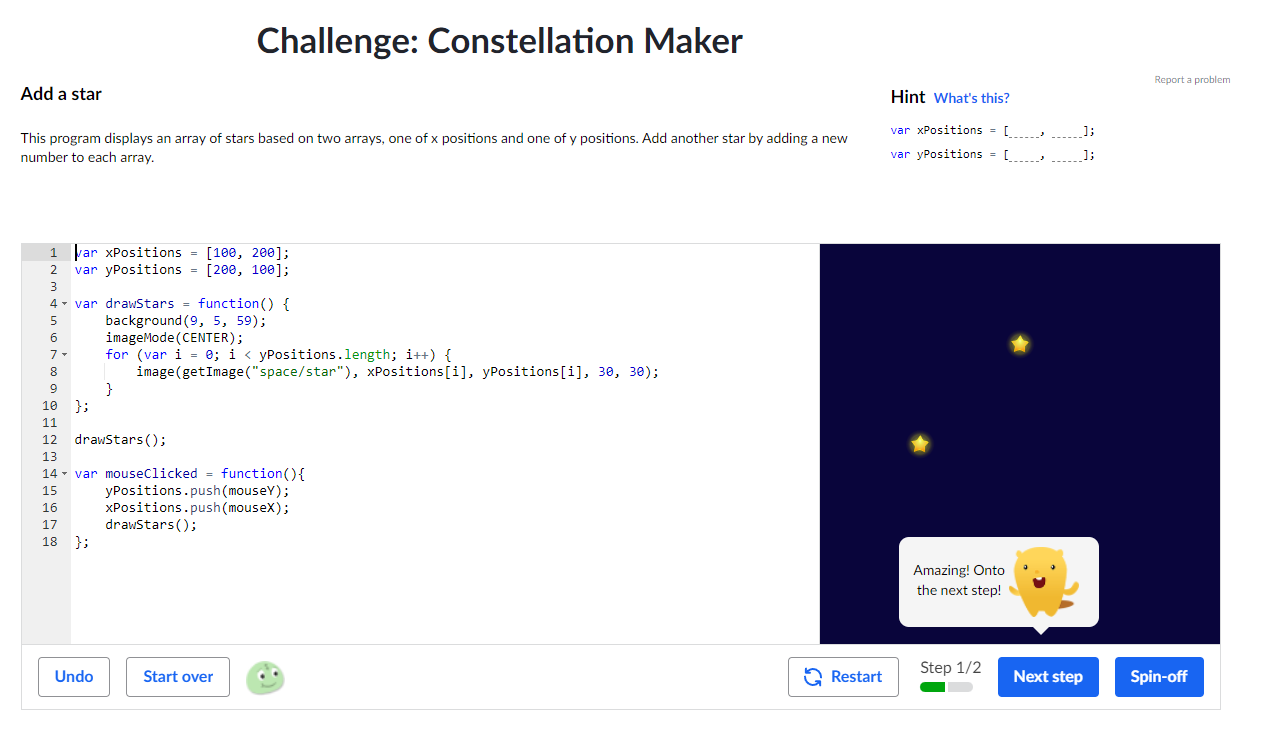
\includegraphics[width=1\linewidth]{assets/similar-games/khanacademy.png}
    \caption{Khan Academy~\cite{a2022_khan}}
    \label{fig:khanacademy}
\end{figure}

Khan Academy is one of the~most extensive generic purpose educational applications with gamification elements.
\textcquote{a2022_khan}{For every student, every classroom. Real results.}
They provide interactive learning materials for math, science, history, economics, etc.
It includes instructional videos supplemented by interactive quizzes and study materials.

After entering the~website, users see all the~Khan Academy's courses.
There are a~vast number of them, and the~courses themselves contain even more individual tasks.
One of the~main focus of the~courses is the~teaching of mathematics, which covers content from primary school, through secondary school, to some topics of university mathematics.

\pagebreak
When clicking on one of the~math courses, the~user is shown a~screen with many units.
On the~side of the~screen, there is also a~summary of the~given units.
That visually represents the~status of the~given parts.
Each unit has several tasks that are either educational, for example, in the~form of text or, more often, video, and several practice tasks that verify the~knowledge gained from the~unit.
The~practice tasks themselves are created visually, and therefore, for example, not only the~example \mintinline{text}|2+3=?| is displayed.
Most of the~time, there is also a~visual representation like two blue boxes and three red ones or marking the~sum on the~axis, etc., according to the~settings of the~given task.

The~application contains the~Computer programming course, which covers an~intro to JS, HTML, CSS, and SQL languages.
The~College Computer Science Principles course covers digital information, the~Internet, cybersecurity, programming, algorithms, simulations, and data analysis.
These courses draw on canvas in JavaScript or do websites using HTML and CSS.

Programming tasks often take the~form of challenges, where the~user receives a~text entry, a~small help, and an~editor in which they can write the~solution of the~task.
An example of a~challenge can be seen in the~figure~\ref{fig:khanacademy}.
Such a~challenging task can also have several steps, and the~task automatically recognizes the~completion of the~current part.
After completing the~task, the~user will have a~button to create a~spin-off if they want to improve the~task and engage in the~solution with their creative spirit.

It also provides a~feature to create and manage classes.
Therefore, teachers can create a~class and invite their students to join.
Then, teachers can create assignments and see students' performances, scores, etc.

According to~\cite{a2022_khan}, Khan Academy is available in more than 50 languages and is free to use.
They are partnered with several schools in the~United States.
And they have more than 130 million registered users in more than 190 countries.
For kids aged 2 to 8, there is also a~learning game-like application called Khan Academy Kids that provides a~joyful and engaging learning curriculum for young children.

\section{CodeCombat}
\label{similar-games:code-combat}

\begin{figure}
    \centering
    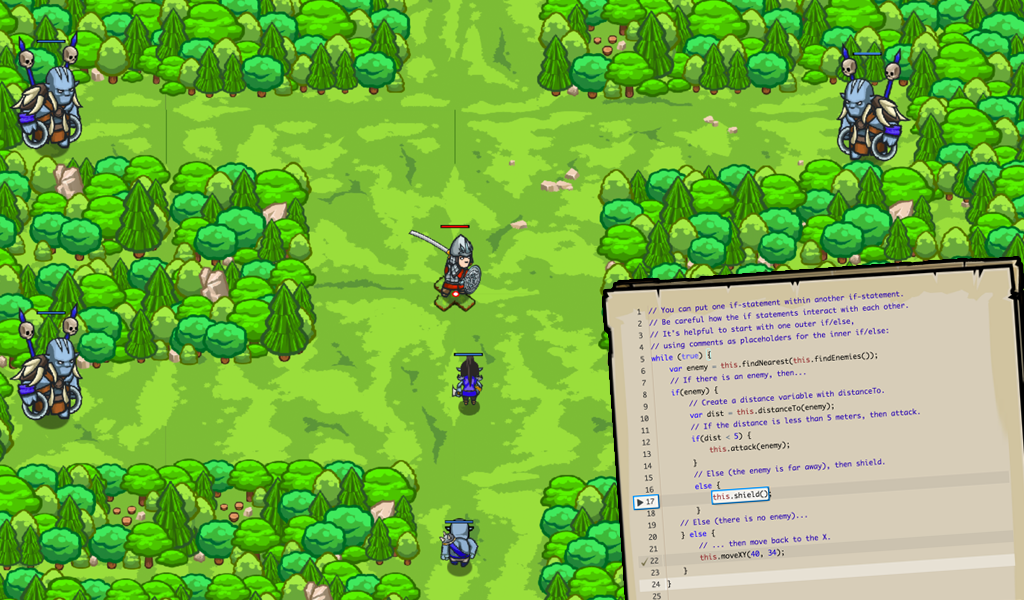
\includegraphics[width=1\linewidth]{assets/similar-games/codecombat.png}
    \caption{CodeCombat~\cite{a2022_codecombat}}
    \label{fig:codecombat}
\end{figure}

CodeCombat is one of the~representatives of a~very story-driven game in which the~player controls a~character through programming.
It is a~community project where volunteers create levels and add features.
Players have their characters with stats and items that add new features to the~player in a~game.

As CodeCombat mentions~\cite{a2022_codecombat}, \textquote{Programming is magic.}
They provide wizard-like features to players so they can use their pure imagination to solve game missions.
And according to the~game, this approach enables players to learn faster.

After entering a~game, the~player sees several game maps.
However, the~player often has to finish the~previous ones to make them available.
The~novice player has the~first game map at his disposal, which guides the~player through the~basic concepts of programming and controlling the~game itself.
Each map includes a~path that intersects the~points that contain game missions.
The~player must pass these points gradually.
The~whole game is styled in a~medieval RPG style, as can be seen in the~figure~\ref{fig:codecombat}.

After starting the~game mission, the~player sees the~playing area and the~goals they must meet.
In addition, the~window may also display smaller help.
In the~corner of the~game, the~goals are displayed, which are marked if the~player has met them.
After completing the~mission, a~dialog box will appear where the~player will be credited with experience points.

The~player can choose one of several languages for programming: Python, JavaScript, CoffeeScript, and Lua.
Languages C++ and Java are available for subscribers.
The~player can play as one of several avatars, each with different abilities and skills.
Some are warriors, others are archers, and others are mages.

Optional missions are also shown on the~map, but they are only accessible to subscribers.
The~player can get a~more extensive selection of avatars and access to more than 500 missions for a~subscription.

\pagebreak
\section{Minecraft}
\label{similar-games:minecraft}

\begin{figure}
    \centering
    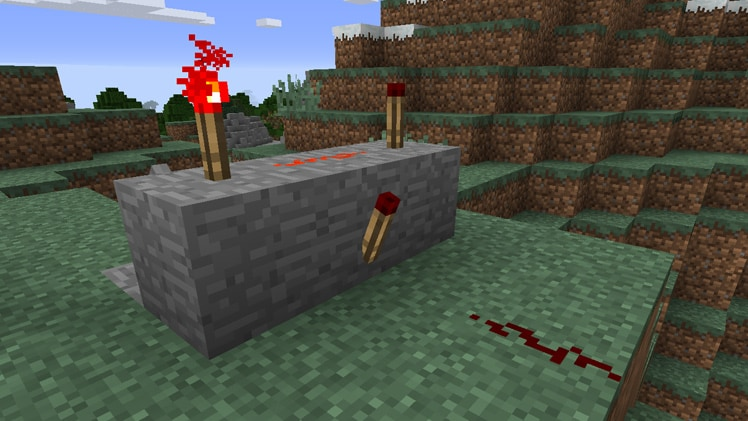
\includegraphics[width=1\linewidth]{assets/similar-games/minecraft.jpg}
    \caption{Minecraft~\cite{a2022_minecraft}}
    \label{fig:minecraft}
\end{figure}

Minecraft is the~most famous building game.
Its minimalistic graphics, where all worlds are made of cube blocks, support creative thinking and creating experiences~\cite{a2022_minecraft}.
It also has an~Education Edition, which focuses on generic purpose education.
That means people can play or create different educational content in the~Minecraft world for any subject.
Both Minecraft Education Edition and Minecraft have ways of introducing programming to children.
Minecraft costs about €24, and anyone can play education Edition with a~Microsoft 365 account.

Minecraft is mainly a~building game.
However, builders also want to build interactive buildings or automate things, so there is Redstone powder in the~game, as can be seen in the~figure~\ref{fig:minecraft}.
That is an~entity that can be placed on blocks and is used to transmit a~signal.
The~game also provides several blocks and entities that can work with the~signal.
These can be, for example, basic buttons and sensors, but also an~archery target, a~light sensor, a~music block, and more.

Some blocks can transmit a~redstone signal, others can receive, and some can do both.
The~restone signal gradually loses its power over the~distance travelled.
The~signal loses all power when more than 15 blocks from the~source.
The~game also includes a~redstone repeater and comparator to manipulate the~redstone signal.
A repeater is a~block used to repeat the~total signal strength and can also delay the~signal or determine the~direction of the~signal.
A comparator is a~block that can compare or subtract signals.

\pagebreak
Other special blocks are, for example, a~piston that can move blocks.
These and other special blocks give players of this game quite versatile programming skills.
The~only downside may be that the~blocks have to be physically placed, and the~design of such a~redstone circuit can be very complicated.

Minecraft Education Edition is a~version of Minecraft designed for schools and education.
It is no longer primarily intended for open-world exploration but more for exploring created learning missions or creating worlds through programming.

The~Code Builder tool is used for programming, in which the~player can program an~agent that executes commands for them.
The~agent is programmed either in JavaScript or using Scratch-style visual programming.
The~agent can do every type of action an~ordinary player would be able to do.

Another option in Minecraft Education Edition is the~Chemistry Lab, where players can get acquainted with the~elements and their creation, compounds, etc.
With this feature, players can learn chemistry and have interactive school lessons.

Minecraft is very popular due to the~modding.
That means players can develop unique modes to customize the~world and game mechanics.
For example, developers can create a mod that adds Pokemons to expand the~Minecraft world.

\begin{figure}
    \centering
    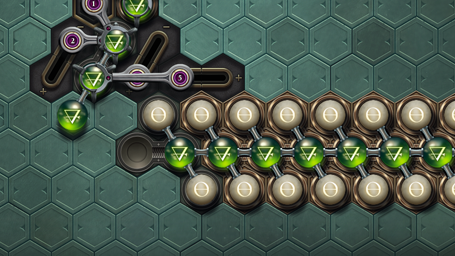
\includegraphics[width=1\linewidth]{assets/similar-games/opusmagnum.png}
    \caption{Opus Magnum~\cite{a2022_zachtronics}}
    \label{fig:opusmagnum}
\end{figure}

\pagebreak
\section{Opus Magnum}
\label{similar-games:opus-magnum}

Opus Magnum is an~exciting game that takes place in an~alchemical world.
According to~\cite{a2022_zachtronics}, the~player's goal is to assemble potions, move them, transmute them, etc., to complete open-ended puzzles.
The~game contains a~transmutation engine.
This engine allows players to place machines that operate according to a~program.
An example of the~game can be seen in the~figure~\ref{fig:opusmagnum}.

In each mission, the~player must produce a~specific alchemical product.
They achieve this using the~transmutation engine.
The~player places elements and components in the~game and uses them to try to produce the~targeted product.
The~game is divided into hexes, and arms are used to move the~elements.
Arms can rotate and move elements closer or further.
There are several types of arms, some of which can handle only one element, some of which can hold more than one element at a~time.
There are also tracks in the~game that can transport elements by rail.
And glyphs that can join elements together or transform into another element.

These mechanical parts are controlled by programming.
At the~bottom of the~game is a~panel with programmable sequences.
According to the~sequences, mechanical parts are controlled.
Players can also compete with each other in three criteria.
One is the~total price, where each mechanical part costs a~certain amount of money.
The~second is the~area of the~table that the~player's machine took.
And the~third is the~number of actions that the~player's machine has performed.
The~game shows histograms and individual statistics among friends on Steam (a game distribution service) for these three criteria.
Players are challenged to make their engines smaller and faster and embrace symmetry and infinity.
The~game also contains a~solitaire minigame.

The~game's background contains a~sophisticated story with other alchemists and the~city's ancient Houses, where the~game missions occur.
The~story also introduces the~basic concepts necessary to understand the~game.
The~graphics are situated in the~dark world of alchemists.
Although the~graphics are excellent, novices or children could have problems with the~game's programming mechanics in the~beginning.
A good element is providing feedback on cost, cycles, and area statistics in which friends can compete.
The~game is not free; it costs around €16.

The~game, according to~\cite{a2022_zachtronics}, provides a~puzzle editor.
Players can use it to create their game missions.
These can then be saved to the~Steam Workshop, and other players and their friends can play the~player's mission.

\pagebreak
\section{7 Billion Humans}
\label{similar-games:7-billion-humans}

\begin{figure}
    \centering
    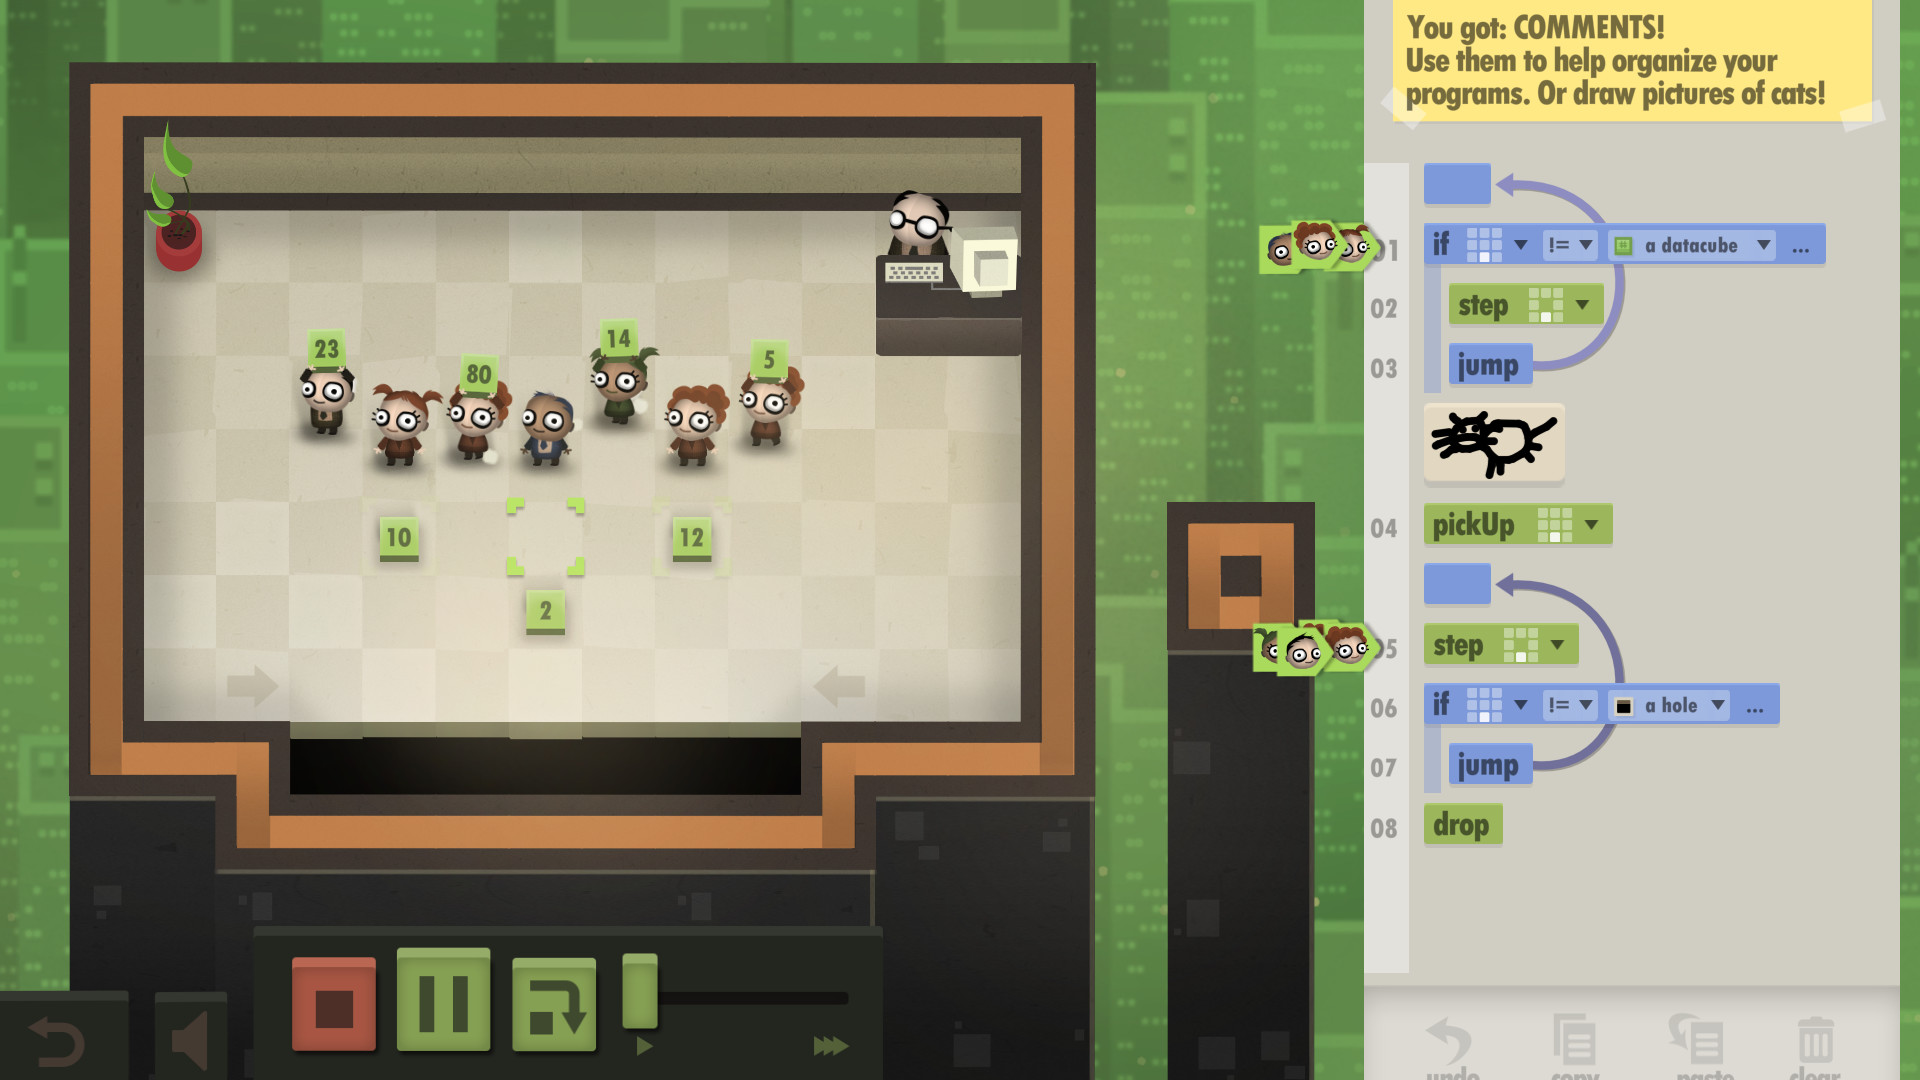
\includegraphics[width=1\linewidth]{assets/similar-games/7bilionhumans.jpg}
    \caption{7 Billion Humans~\cite{a2022_tomorrow}}
    \label{fig:7bilionhumans}
\end{figure}

7 Billion Humans is a~puzzle game where your task is to program a~parallel computer made of people, as can be seen in the~figure~\ref{fig:7bilionhumans}.
Therefore, the~player's job is to the~figure out how to synchronize workers to achieve the~expected outcome.

The~players are presented with simple, stylish graphics.
Players have to solve programming puzzles, and each game mission has a~specific task.
They have human workers who follow the~visual commands.
Data cubes are often used in tasks.

Interestingly, the~same program is used to program all human staff at once.
Of course, each employee works with the~program individually according to their surroundings and internal logic.
That requires players to engage in wit in creating such a~sequence of commands to make the~game come true.

According to~\cite{a2022_tomorrow}, once the~player comes up with a~working solution, the~game performs another 25 cases in which they randomly exchange data like in the~data cubes, thus testing the~quality of the~solution.
Optional game tasks are overcoming the~average number of steps and average time.
This concept motivates players to optimize programs.

The~biggest drawback for inexperienced players might be that the~game does not explain the~concepts.
But the~concepts are simple so that players can get into it quickly.
The~game costs around €12.

\section{Codewars}

\begin{figure}
    \centering
    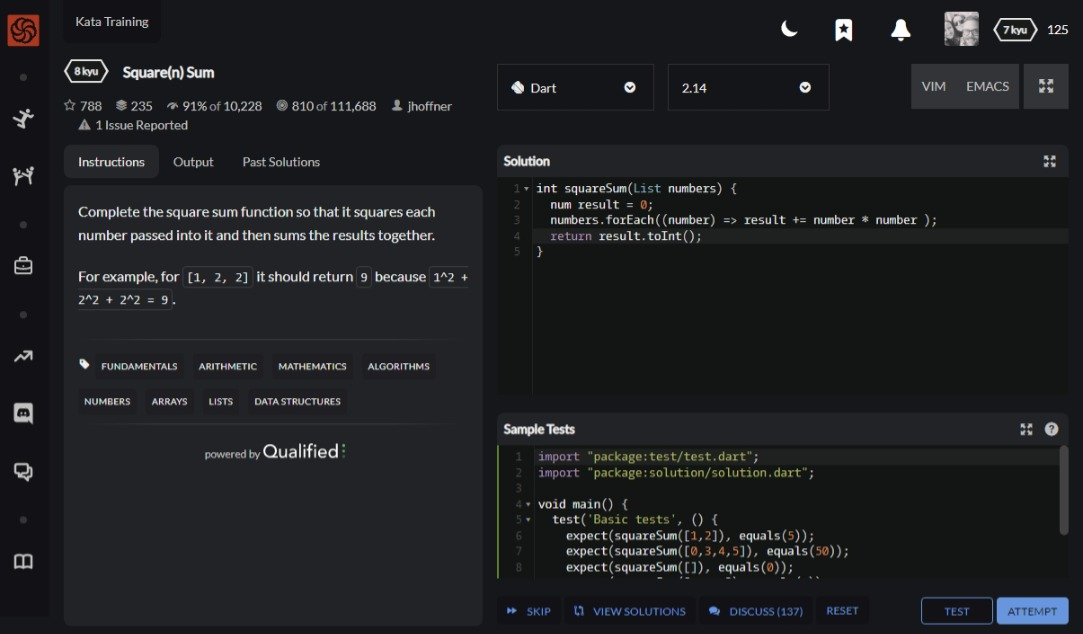
\includegraphics[width=1\linewidth]{assets/similar-games/codewars.jpeg}
    \caption{Codewars~\cite{a2022_codewars}}
    \label{fig:codewars}
\end{figure}

Codewars is a~game that provides a~place for independent tasks.
The~game has no story or fixed order of tasks.
Instead, the~tasks have tags that distinguish their focus, and the~player himself chooses the~engaging exercises they want to play.
That makes this game very unique.

These tasks, which are code challenges, are called \textquote*{kata}.
Each kata has a~Kyu/Dan rank, indicating its difficulty.
According to~\cite{a2022_codewars}, these terms are borrowed from Japanese martial arts.
The~master level is called Dan, and Kyu indicates the~number of levels from that level.
Beginners thus have 8~kyu.
Conversely, the~best grade is 4~dan.
Each player has a~Kyu/Dan rating, and the~player progresses when they complete the~kata of the~same or higher level.

In addition, the~game has an~honor system, which is obtained by creating a~kata, constructive commentary, and promising solutions.
This system is therefore based on community evaluation.
Together, these concepts form a~fascinating combination in teaching, similar to martial arts.

The~player can use over 20 programming languages such as Python,\linebreak{}JavaScript, etc.
Each kata has its description and instructions, where the~player learns what the~task is focused on.
Players also see sample tests that the~generated code must pass.
Then the~players try to write a~code that will meet the~requirements.
If players do not know how to complete a~kata, they can unlock a~reference solution, but that will deprive them of the~opportunity to gain a~kata rank or honor.
They can also open a~discussion to ask about problems or other advice.
A sample of the~kata screen can be seen in the~figure~\ref{fig:codewars}.

\pagebreak
Katas are met by passing tests.
If the~player programs a~solution, they can test it against the~sample input.
These usually cover units of simple cases.
Once these tests are completed, the~code can be tested on a~larger sample of tests and then submitted.

Codewars is suitable for getting out of players' comfort zone.
Individual katas are challenging, cover a~variety of cases, and allow players to try new things and approaches.
Players can also learn a~new programming language that they can try out in practice and even create solutions in multiple languages.
Some katas require geometry and algebra, which players will also repeat.
And one of the~most beneficial uses is the~opportunity to learn from the~solutions of others.
And of course, compete and compare with friends. 

\section{CodeMonkey}

\begin{figure}
    \centering
    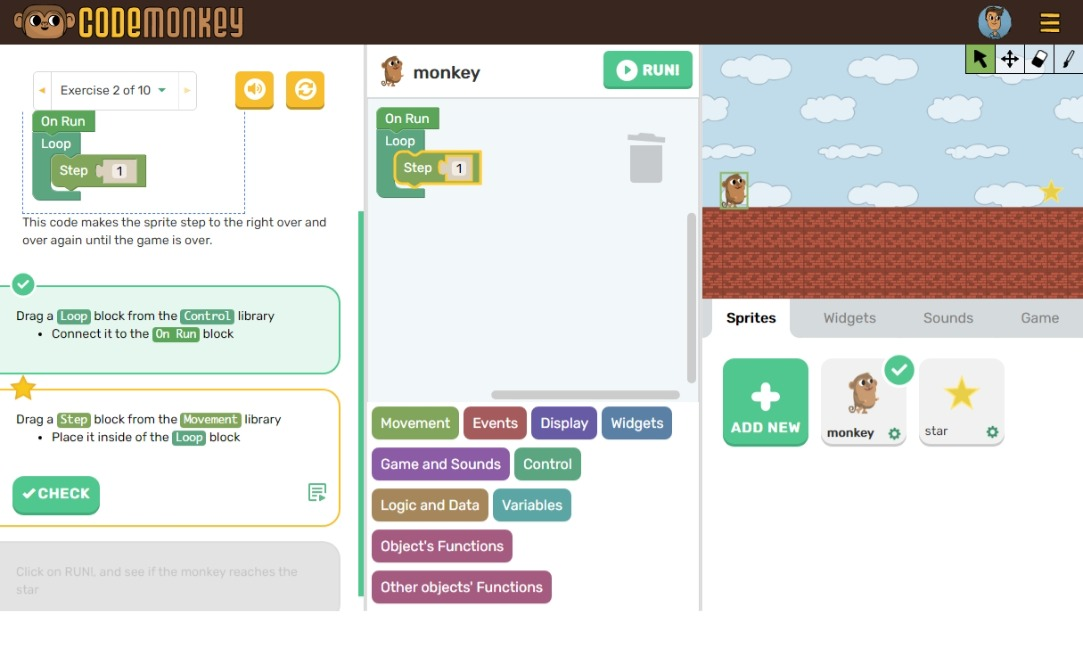
\includegraphics[width=1\linewidth]{assets/similar-games/codemonkey.jpeg}
    \caption{CodeMonkey~\cite{a2020_codemonkey}}
    \label{fig:codemonkey}
\end{figure}

CodeMonkey is a~game focused on teaching programming to children.
The~game contains several separate courses, each with a~different story and a~different form of programming.
Simplified visual programming with picture boxes is available for the~youngest children and beginners.
Other courses then use visual programming blocks similar to Scratch.
And other more advanced courses use text programming using Python or CoffeeScript.
The~game provides students with various educational resources that provide learning material for the~youngest to the~oldest.

\pagebreak
According to~\cite{a2020_codemonkey}, CodeMonkey provides classroom support for schools in which students can be managed.
The~teacher sees the~statistics, can assign tasks and can set up an~automatic evaluation.
The~game is used by over 25 million students and over 120,000 teachers.
Of course, the~game can be played as an~individual outside of school, from home comfort.
The~game also supports web and mobile applications, making it accessible to most players.

After logging in to the~game, the~user sees many available courses.
Each is marked for beginners, beginners, intermediate or advanced.
It also indicates which method is used for programming: block coding, text coding, etc.
Players will see a~slightly different game window based on the~method used.
Usually, however, the~player has a~command panel, whether in visual or textual form, and a~game panel.
The~assignment is displayed to the~player in the~panel itself or is gradually communicated using dialog boxes.
Game missions with block coding in a~version similar to Scratch also have progressive goals that are marked if the~user accomplishes them.
Each goal also has advice on how to meet them.
The~player can use various sprites, widgets, sounds, and command blocks in this Scratch-like environment.
An example of the~game mission can be seen in the~figure~\ref{fig:codemonkey}.

As in Scratch, players can create their games using text or visual programming.
However, the~game builder editor is only available to subscribers.
Players can see the~creations of others, which they can also try, evaluate and remix.

The~game includes ten free courses but includes an~additional twenty-one for subscription players.
The~cheapest individual license costs about \$6 per month.
Unique school plans are available for schools, which must be agreed upon individually.

\section{Codemancer}

\begin{figure}
    \centering
    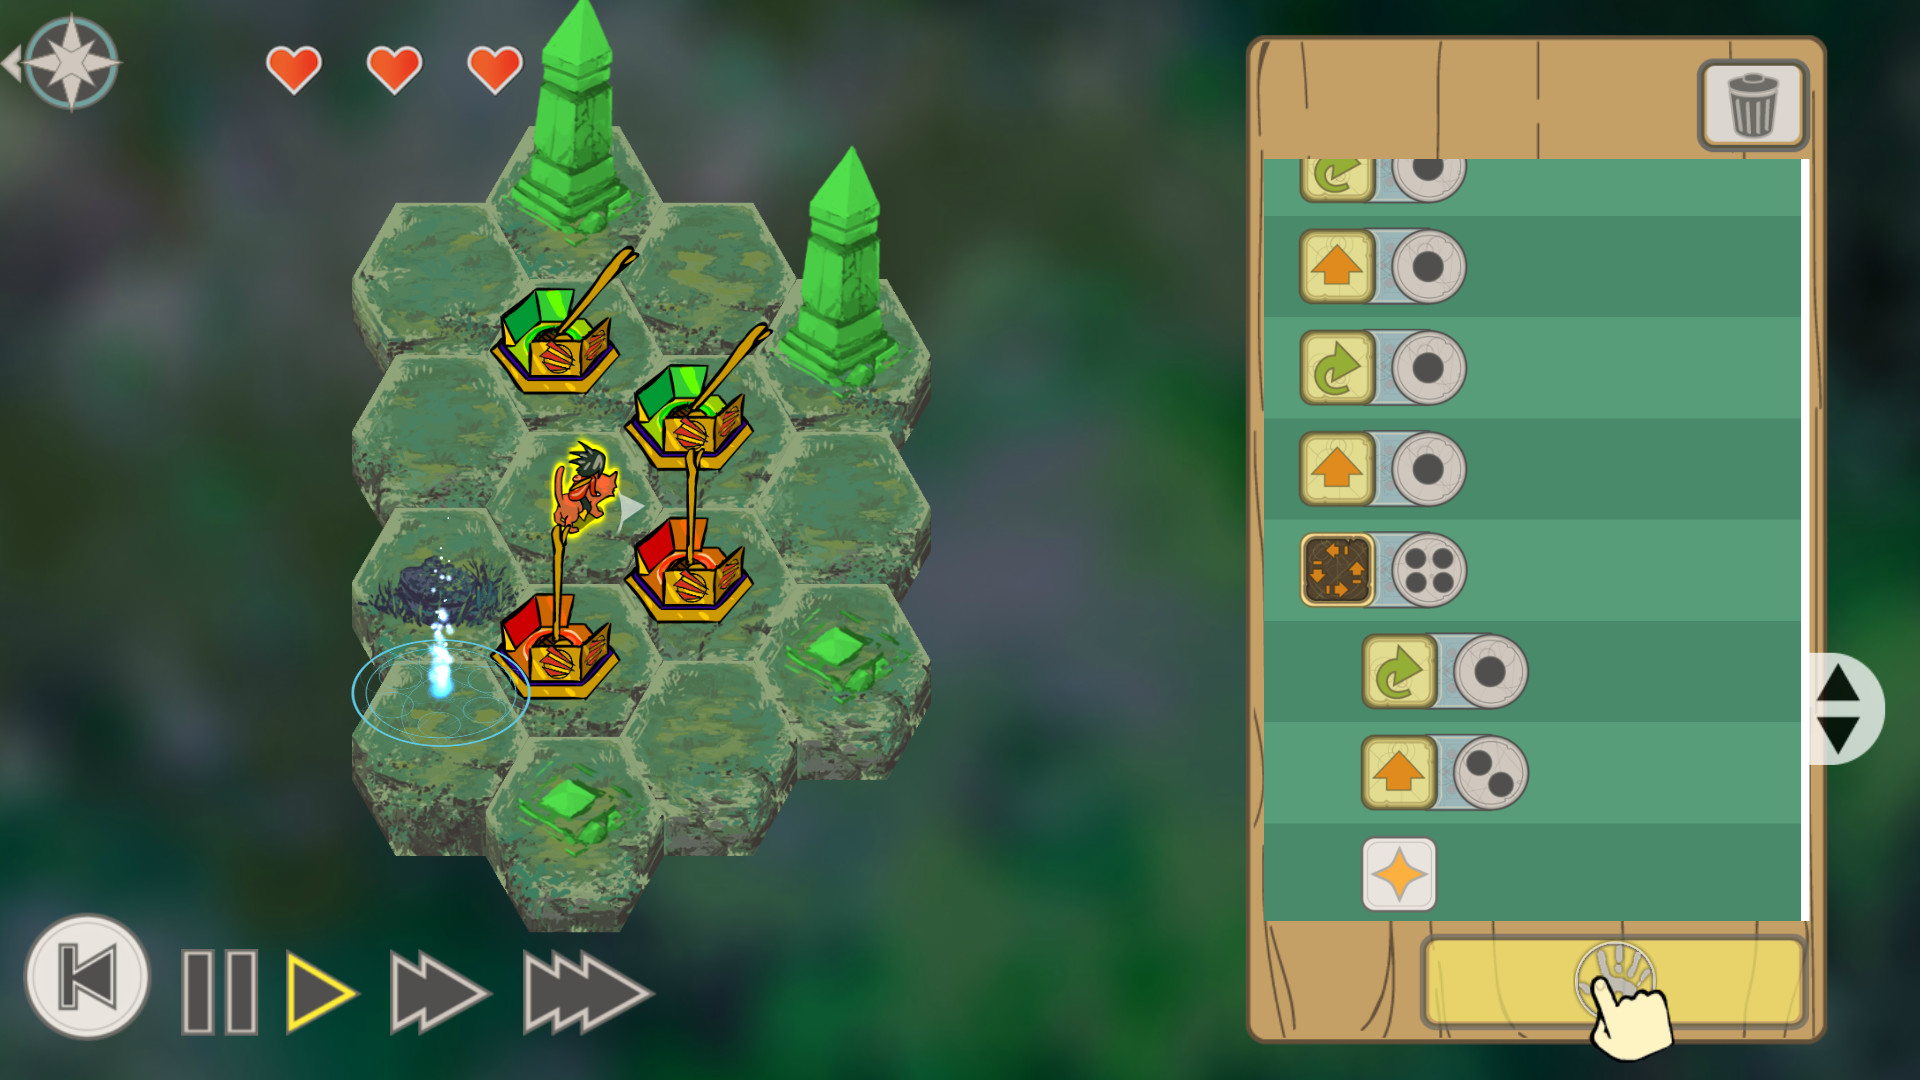
\includegraphics[width=1\linewidth]{assets/similar-games/codemancer.jpg}
    \caption{Codemancer~\cite{a2021_codemancer}}
    \label{fig:codemancer}
\end{figure}

Codemancer is an~educational game that teaches programming to children.
\textcquote{a2021_codemancer}{A fantasy game that teaches the~magic of code,} as stated by their site.
According to~\cite{a2021_codemancer}, the~game is aimed at children aged 6 to 12.
It has a~moving fantasy story that is a~big part of the~game.
The~story revolves around a~little girl Aurora, who is trying to grow up and is facing obstacles.
The~girl must learn the~magic with which she must save her father.

In the~game, players use commands in the~form of special runs.
These runes can be modified in an~attached box, where the~player can usually select the~number of repetitions.
Typically, the~player selects a~rune to move and modifies its number so that, for example, the~character moves three times.
Similarly, it can modify the~rotation rune.
The~game takes place on a~hexagonal grid, on which is the~player's character, the~girl Aurora, whom the~player controls, as can be seen in the~figure~\ref{fig:codemancer}.

An exciting concept is how the~steps are performed.
The~player does not have to set all the~steps immediately but can perform graduate sequences one after the~other.
The~character can rotate one hex to the~right and take two steps forward, and in the~following sequence, they can turn left and take action.
That adds an~exciting aspect of gradual development to the~game.
As the~game progresses, the~game shows players new programming concepts such as cycles, variables, conditions, and functions. 

The~game is available on mobile devices and desktops.
It is available for free at the~Steam store, which distributes the~game for desktops, and the~App Store distributes the~game on Apple devices.
The~Google Play store, which distributes the~game on Android, is available for about €5.

\section{Baba Is You}

\begin{figure}
    \centering
    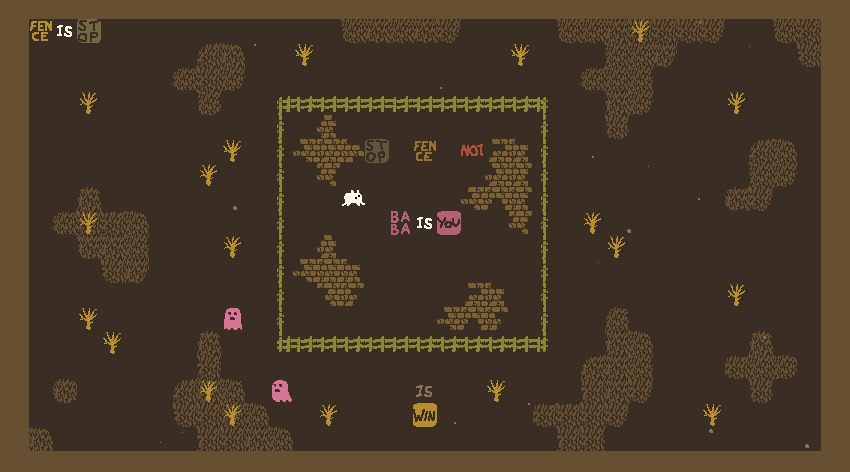
\includegraphics[width=1\linewidth]{assets/similar-games/baba.png}
    \caption{Baba Is You~\cite{a2022_baba}}
    \label{fig:babaisyou}
\end{figure}

Baba Is You is a~very different game.
While in previous games, players create sequences using blocks or by writing code, in this game, the~game itself programs the~game.
The~game character can move blocks that are composed of text.
These text blocks can create another combination, such as allowing a~character to walk through a~wall or change a~character to another object, even to a~wall.

According to~\cite{a2022_baba}, the~game relies on manipulating the~rules that are part of the~game, and the~player's goal is to change and abuse these rules to their advantage.
The~game has simple pixel graphics that add a~pleasant atmosphere, as can be seen in the~\ref {fig:babaisyou}.
The~mechanics themselves, where the~rules are incorporated into the~game itself, and the~game is governed by changing rules, is an~exciting way for one to improve in problem-solving.

The~object of the~game may be, for example, to touch a~flag that signifies victory in a~given mission; if the~rules of the~game mention it.
But the~problem is how to get to the~flag.
In addition, the~game map consists of several walls, rooms, and other blocks that the~character cannot pass.
Touching some blocks can mean a~defeat.
The~player's goal is to find such game rules and modifications so that the~player reprograms the~game and wins the~mission.

The~game is available on Windows, Linux, and macOS desktops for around \$15.
The~game contains over 200 levels that players can play.

\section{Evaluation}

All the~mentioned games have fascinating concepts and mechanics, thanks to which players, and therefore children, can improve their programming skills.
However, none are available for free (without significant restrictions), contain an~exciting and engaging story, and provide study materials.
Therefore a~game with gamification features mentioned in chapter~\ref{analysis} will be designed and implemented.

Each game has unique features by which the~proposed game can be inspired.
Scratch has tools for creative game development using visual programming and promotes healthy competitiveness, but it is not very focused on teaching and story.
Khan Academy has an~extensive curriculum and many challenges, but it is not focused on the~story.
CodeCombat has an~exciting story and, with the~help of excellent graphics, allows children to learn to program, but the~free version can be limited in time.
Minecraft has a~uniquely integrated programming feature to the~in-game world, but it focuses on exploring and creating worlds rather than on teaching and the~story itself.
Opus Magnum has joyful visual programming tools with an~engaging, mysterious story in the~background, but not available for free.
7~Billion Humans is an~exciting game with nice graphics and parallel programming, but it lacks a~deeper story and teaching materials.
CodeWars is more suitable for self-study with challenges than teaching with a~plan.
CodeMonkey contains a~wide variety of programming missions and various programming approaches, but the~options of the~free version are limited.
Codemancer is partially free and provides an~exciting story around which the~whole game revolves, but more complex concepts are not much explained, and the~game is more suitable for more minor children.
And Baba Is You is a~great-looking and exciting game, but it is more suitable for practicing problem-solving than teaching programming.

The~designed game should incorporate all these games' benefits into itself.
The~game should have good storytelling, create a~joyful visual programming tool that can be easily understood by children, and provide a~way how players can learn basic and advanced concepts. 
The~proposed game should also be accessible and open-source to provide its content to students for free while making the~code available to other developers who may be looking for inspiration.